\section*{Глава 3\\Численный метод}
\addcontentsline{toc}{section}{Глава 3. Численный метод}
\setcounter{section}{3}
\setcounter{subsection}{0}
\setcounter{equation}{0}

\subsection{Расщепление по направлениям}

	Чтобы решить систему уравнений:
\begin{equation}
	\label{matrix_anisotropy_equation1}
	\frac{\partial\vec{u}}{\partial{t}}+\mathbf{A}_x\frac{\partial\vec{u}}{\partial{x}}+
	\mathbf{A}_y\frac{\partial\vec{u}}{\partial{y}}+
	\mathbf{A}_z\frac{\partial\vec{u}}{\partial{z}}=0
\end{equation}
	методом конечных разностей потребывалось записать бы это уравнение на некотором сеточном шаблоне в каждом узле сетки, а затем решать полученную линейную систему.
	Решение этой системы, состоящей из огромного количества переменных представляется очень сложной задачей.
	С другой стороны вид системы \eqref{matrix_anisotropy_equation1} позволяет нам применить метод дробных шагов для её решения, сводя её, таким образом, к одномерной постановке:
\begin{equation}
	\label{norm_form}
	\frac{\partial\vec{u}}{\partial{t}}+\mathbf{A}_x\frac{\partial\vec{u}}{\partial{x}} = 0
\end{equation}

	Запишем для уравнения \eqref{norm_form} соотношение между искомым вектором на следующем временном слое $\vec{u}^{n+1}$ и на текущем $\vec{u}^{n}$ через оператор перехода между слоями $f$ в виде:
\begin{equation}
	\label{simple_splitting}
	\vec{u}^{n+1} = f_x(\mathbf{A}_x)\vec{u}^{n}.
\end{equation}	
	
	Тогда, в простейшем случае, окончательные выражение для $\vec{u}^{n+1}$ будет:
\begin{equation}
	\label{simple_3D_splitting}
	\vec{u}^{n+1} = F(\mathbf{A}_x, \mathbf{A}_y, \mathbf{A}_z)\vec{u}^{n},
\end{equation}
\begin{equation}
	\label{simple_3D_split_operator}
	F(\mathbf{A}_x, \mathbf{A}_y, \mathbf{A}_z) = \alpha_x f_x(\frac{\mathbf{A}_x}{\alpha_x}) + \alpha_y f_y(\frac{\mathbf{A}_y}{\alpha_y}) + \alpha_z f_z(\frac{\mathbf{A}_z}{\alpha_z}).
\end{equation}
	
	При условии, что за $f_x$, $f_y$, $f_z$ взяты разностные схемы, аппроксимирующие соответствующие уравнения вида \eqref{norm_form}, как минимум первого порядка точности по пространству, а также при выполнении условия:
\begin{equation}
	\label{simple_3D_split_cond}
	\alpha_x + \alpha_y + \alpha_z = 1, \quad \alpha_x, \alpha_y, \alpha_z > 0,
\end{equation}
	схема \eqref{simple_3D_splitting} с оператором \eqref{simple_3D_split_operator} обеспечивает первый порядок точности.
	Такой подход, комбинирующий сочетания решений одномерных систем, носит название \textit{расщепление по направлениям} \cite{chelnokov}.
	
	Ограничение на шаг по времени $\tau$, обеспечивающее устойчивость дальнейшего численного решения, будет иметь вид:
\begin{equation}
\tau \le \max{\tau_j} = \frac{\min(h)}{\max(|\lambda_j^*|)} = \frac{\min(h)\alpha_j}{\max(|\lambda_j|)},
\end{equation}
	где $\lambda_j$ -- собственные значения матриц $\mathbf{A}_x$, $\mathbf{A}_y$, $\mathbf{A}_z$.
	
	Если за одномерные операторы перехода $f$ взять схемы второго порядка и скомбинировать их в полный оператор:
\begin{equation}
	\label{3D_split_operator}
	F(\mathbf{A}_x, \mathbf{A}_y, \mathbf{A}_z) = \frac{1}{6}\sum_{i \neq j \neq k \neq i} f_i(\mathbf{A}_i)f_j(\mathbf{A}_j)f_k(\mathbf{A}_k),
\end{equation}
	то мы получим схему второго порядка. 
	
	Допустимый шаг по времени определяется минимальным допустимым шагом по времени для схем $f_j$:
\begin{align}
\tau = \min\limits_{j}(\tau_j) = \min\limits_{j}(\frac{\min(h)}{\max(|\lambda_j|)}) = \frac{\min(h)}{\max\limits_{j}\max(|\lambda_j|)}.
\end{align}
	
	Однако вычисления по схеме \eqref{3D_split_operator} требуют больших затрат компьютерного времени и памяти.
	Как оказалось, вычисление любого одного слагаемого из \eqref{3D_split_operator} даёт хорошее приближение к схеме второго порядка, например:	
\begin{equation}
	\label{short_3D_split_operator}
	F(\mathbf{A}_x, \mathbf{A}_y, \mathbf{A}_z) = f_x(\mathbf{A}_x)f_y(\mathbf{A}_y)f_z(\mathbf{A}_z).
\end{equation}
	
\subsection{Гиперболическая система уравнений. Инварианты Римана}
	
	Систему квазилинейных уравнений в частных производных, записанную в \textit{нормальной форме} \eqref{norm_form} будем считать \textit{гиперболической}.
	Это значит, что матрица $\mathbf{A}$ подчиняется условиям\cite{rozhdestvenskiy}:
\begin{itemize}
	\item все собственные значения матрицы $\lambda_{i} = \lambda_{i}(t, x, \vec{u})$, $i = \overline{1, 9}$ вещественны;
	\item система собственных векторов матрицы $\{l_{i}(t, x, \vec{u})\}$, $i = \overline{1, 9}$ образует базис в пространстве $E_{n}$.
\end{itemize}

	В таком случае матрица $\mathbf{A}$ \textit{диагонализуема}, т.е. существует базис -- басиз собственных векторов -- в котором она имеет диагональный вид.
	Тут мы будем говорить о собственных строках $\vec{l}^{T}$, таких, что:
\begin{equation}
	\label{eigenstr_equation}
	\vec{l}^{T}\mathbf{A} = \lambda\vec{l}^{T}.
\end{equation}
	
	Итак, матрица $\mathbf{A}$ представима в виде:
\begin{equation}
	\label{diagonal_view}
	\mathbf{A} = \mathbf{\Omega}^{-1}\mathbf{\Lambda}\mathbf{\Omega},
\end{equation}	
	где $\mathbf{\Omega}$ -- матрица собственных строк, $\mathbf{\Lambda}$ -- диагональная матрица собственных значений.
	Тогда умножая справа \eqref{norm_form} на $\mathbf{\Omega}$ получим:
\begin{equation}
	\label{norm_form1}
	\mathbf{\Omega}\frac{\partial\vec{u}}{\partial{t}}+\mathbf{\Lambda}\mathbf{\Omega}\frac{\partial\vec{u}}{\partial{x}} = 0.
\end{equation}
	Далее, если компоненты матрицы $\mathbf{\Omega}$ не зависят от переменных $(x, t)$, то её можно внести под знак дифференцила:
\begin{equation}
	\label{norm_form2}
	\frac{\partial(\mathbf{\Omega}\vec{u})}{\partial{t}}+\mathbf{\Lambda}\frac{\partial(\mathbf{\Omega}\vec{u})}{\partial{x}} = 0.
\end{equation}
	В общем случае, когда $\mathbf{\Omega} = \mathbf{\Omega}(x, t, \vec{u})$, $\mathbf{\Lambda} = \mathbf{\Lambda}(x, t, \vec{u})$ можно попробывать поискать интегрирующий множитель, однако для системы девяти уравнений это проблематично.
	
	Обозначая, $\vec{r} = \mathbf{\Omega}\vec{u}$ получим уравнение:
\begin{equation}
	\label{Riman_invariantes}
	\frac{\partial\vec{r}}{\partial{t}}+\mathbf{\Lambda}\frac{\partial\vec{r}}{\partial{x}} = 0.
\end{equation}
	Или же в такой форме \cite{kukudzhanov_main}:
\begin{equation}
	\label{Riman_invariantes1}
	\left(\frac{dr_k}{dt}\right)_k = 0, \quad k = \overline{1, 9},
\end{equation}
	где $r_k$, компоненты вектора $\vec{r}$ называются \textit{инвариантами Римана}, а система \eqref{Riman_invariantes} \textit{системой в инвариантах}.
	В записи \eqref{Riman_invariantes} введено обозначение:
\begin{equation}
	\label{notation}
	\left(\frac{d}{dt}\right)_k = \frac{\partial}{\partial{t}} + \lambda_k \frac{\partial}{\partial{x}}
\end{equation}
	Это оператор дифференцирования вдоль направления, заданного уравнением:
\begin{equation}
	\label{characteristic_direction}
	\frac{dx}{dt} = \lambda_k, \quad k = \overline{1, 9}.
\end{equation}
	Уравнения \eqref{characteristic_direction} -- уравнения на \textit{характеристики} системы \eqref{norm_form} -- интегральные кривые вдоль которых инварианты $r_k$ постоянны. 
	
	Эти рассуждения лежат в основе \textit{метода характеристик} -- метода решения систем гиперболических уравнений, в котором решение уравнений в частных производных сводится к решению обыкновенных дифференциальных уравнений (ОДУ).
	В свою очередь, для численного решения ОДУ могут быть применены стандартные конечно-разностные схемы. Такой подход составляет суть \textit{сеточно-характеристического метода}. 
	
\subsection{Cеточно-характериситческий метод}

	Гиперболические уравнения описывают распространение различного типа волн в средах.
	Простейшим решением одномерного волнового уравнения являются две волны: $f(x \pm vt)$, распространяющиеся в противоположных направлениях.
	Функция $f$ -- вид начального возмущения, как можно видеть, параметризованная указаным образом, она даёт решение уравнения.
	Важным здесь является то, что некоторые линейные комбинации искомых величин сохраняются на определённых пространственно-временных кривых (характеристиках).

\begin{figure}[H]
	\center{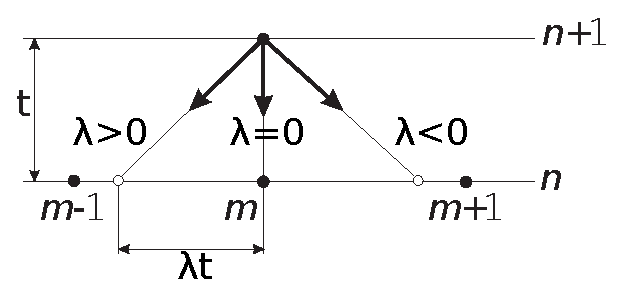
\includegraphics[width=0.5\textwidth]{png/gcm-idea.eps}}
	\caption{Принципиальная схема сеточно-характеристического метода.}
\end{figure}

	После расщепления наша система предстаёт в виде трёх гиперболических систем, описывающих распространение продольной и двух поперечных волн вдоль каждой оси (всего вдоль каждой оси распространяется шесть волн -- с положительными и отрицательными скоростями).
	Затем, переходя к инвариантам, мы получаем девять уравнений переноса вдоль каждой оси.
	Решение этих уравнений сеточно-характеристическим методом осуществляемся следующим образом:
\begin{enumerate}
	\item Из узлов сетки на очередном временном слое проводятся характеристики на предыдущий временной слой (см. Рис. 2). Для линейной системы уравнений характеристиками будут семейства параллельных прямых.
	\item Находятся точки пересечения характеристик с предыдущим временным слоем.
	\item В этих точках, применяя различные схемы, производится интерполяция искомых функций (на Рис. 2 изображён трёхточечный шаблон).
	\item По найденным значениям производится пересчёт инвариантов, которые переносятся по характеристикам в исходный узел.
\end{enumerate}
	
	Как уже сказано характеристики -- прямые линиии постоянного наклона. Это значит можно точно решить уравнение на характеристики \eqref{characteristic_direction}, поэтому определяющим фактором здесь является интреполяция инвариантов.
	Схема интерполяции второго порядка с разностями против потока (upwind scheme) является здесь предпочтительной.
	При числе Куранта в близкой окрестности единицы эта схема может оказаться особенной точной.
	
	В итоге инварианты на $(n+1)$-ом временном слое можно записать в виде:
\begin{equation}
	r_{i}^{n+1} = r_{i}^{n}(- \lambda_{i}\tau),
\end{equation}
	где $r_{i}$ -- $i$-ый инвариант Римана, $\lambda_{i}$ -- соответствующее ему собственное значение.
	Такая запись означает, что значение инварианта $r_{i}$ берётся на $n$-ом слое в точке смёщённой на $-\lambda_{i}\tau$ от координаты искомой.
	
	Затем искомый $\vec{u}$ вектор находится по формуле:
\begin{equation}
	\vec{u} = \mathbf{\Omega^{-1}}\vec{r}.
\end{equation}	

\subsection{Разностные схемы для структурированных сеток}
	
	Существует множество готовых расностных схем для решения уравнения \eqref{norm_form}.
	По сути эти схемы аналогичны сеточно-характерестическому методу, использующему различные схемы интерполяции инвариантов на предыдущем слое.
	
\paragraph{Схема Куранта-Изаксона-Рис.} Данная схема строится на трёхточечном сеточном шаблоне $(m-1, m, m+1)$ и позволяет явно выразить значение $\vec{u}_m^{n+1}$ на новом временном слое:
\begin{equation}
	\label{CIR scheme}
	\vec{u}^{n+1}_m = \vec{u}^n_m - \frac{\tau}{h} \mathbf{\Omega}^{-1} \mathbf{\Lambda}^+ \mathbf{\Omega} (\vec{u}^n_{m+1} - \vec{u}^n_m) 
	- \frac{\tau}{h} \mathbf{\Omega}^{-1} \mathbf{\Lambda}^- \mathbf{\Omega} (\vec{u}^n_m - \vec{u}^n_{m-1}) .
\end{equation}
	Здесь диагональные матрицы $\mathbf{\Lambda}^+$, $\mathbf{\Lambda}^-$ содержат соответственно положительные и отрицательные собственные значения (скорости распространения волн).
	
	Эта схема является схемой первого порядка точности по времени и пространству -- $O(h, \tau)$.
	
\paragraph{Схема Лакса-Вендрофа.} Стандартная схема Лакса-Вендрофа обладает вторым порядком точности и по времени и по пространству -- $O(h^2 + \tau^2)$.
\begin{equation}
	\label{LW scheme}
	\vec{u}^{n+1}_m = \vec{u}^n_m - \frac{\tau}{2h} \mathbf{A} (\vec{u}^n_{m+1} - \vec{u}^n_{m-1})
	 + \frac{\tau^2}{2h^2} \mathbf{A}^2 (\vec{u}^n_{m+1} - 2\vec{u}^n_m + \vec{u}^n_{m-1}) .
\end{equation}
	Эта схема в отличие от предыдущей не является монотонной. 
	Схемы, у которых отсутствует свойство монотонности плохо аппроксимируют решения с большими градиентами -- они выдают осцилляции разностного происхождения вблизи области с больши градиентом.
	
\paragraph{Гибридная схема.} Именно для сочетания точности схем второго порядка и устранения осцилляций для решений с большими градиентами Р.П. Федоренко впервые предложил \textit{гибридные схемы} \cite{fedorenko}.
	В нашем случае, комбинируя схему \eqref{CIR scheme} со схемой \eqref{LW scheme}, итоговое решение будет иметь вид линейной комбинации решений двух схем:
\begin{align}
	\label{hybrid scheme}
	\vec{u}^{n+1}_m &= \vec{u}^n_m - \frac{\tau}{2h} \mathbf{A} (\vec{u}^n_{m+1} - \vec{u}^n_{m-1}) + \nonumber\\
		&+ \frac{1}{2} ((1-a) \frac{\tau}{h} \mathbf{\Omega}^{-1} |\mathbf{\Lambda}| \mathbf{\Omega} + a \frac{\tau^2}{h^2} \mathbf{A}^2 ) (\vec{u}^n_{m+1} - 2\vec{u}^n_m + \vec{u}^n_{m-1}).
\end{align}
	Параметр $a$ может принимать значения: $0 \leq a \leq 1$, и подбирается на каждом шагу в зависимости от степени гладкости решения. 
	В случае $a = 0$ схема \eqref{hybrid scheme} переходит в схему Куранта-Изаксона-Рис \eqref{CIR scheme}.
	В случае $a = 1$ схема \eqref{hybrid scheme} переходит в схему Лакса-Вендрофа \eqref{LW scheme}.
	
	Решение уравнения \eqref{norm_form} по схеме \eqref{hybrid scheme} заключается в переключении между схемами \eqref{CIR scheme} и \eqref{LW scheme} в зависимости от гладкости $n$-ого временного слоя.
	Критерий переключения имеет вид:
\begin{equation}
	\label{Fedorenko criterium}
	\left|\frac{\vec{u}^n_{m+1} - 2\vec{u}^n_m + \vec{u}^n_{m-1}}{\vec{u}^n_{m+1} - \vec{u}^n_{m-1}}\right| \le K,
\end{equation}
	где параметр переключения -- $K$ подбирается, опять же, в зависимости от гладкости решения и в данной работе: $K = 0.5$.
	В случае выполнения условия \eqref{Fedorenko criterium} решение считается достаточно гладким, параметр принимает значение: $a = 1$ и расчёт ведётся по схеме Лакса-Вендрофа.
	Если же критерий не выполняется, то $a = 0$ и расчёт производится по схеме Куранта-Изаксона-Рис.
	
	На Рис. 3 изображены несколько численных решений распространения прямоугольного импульса. Как можно отметить гибридная схема лучше остальных приближает точное решение.
\begin{figure}[H]
\centerline{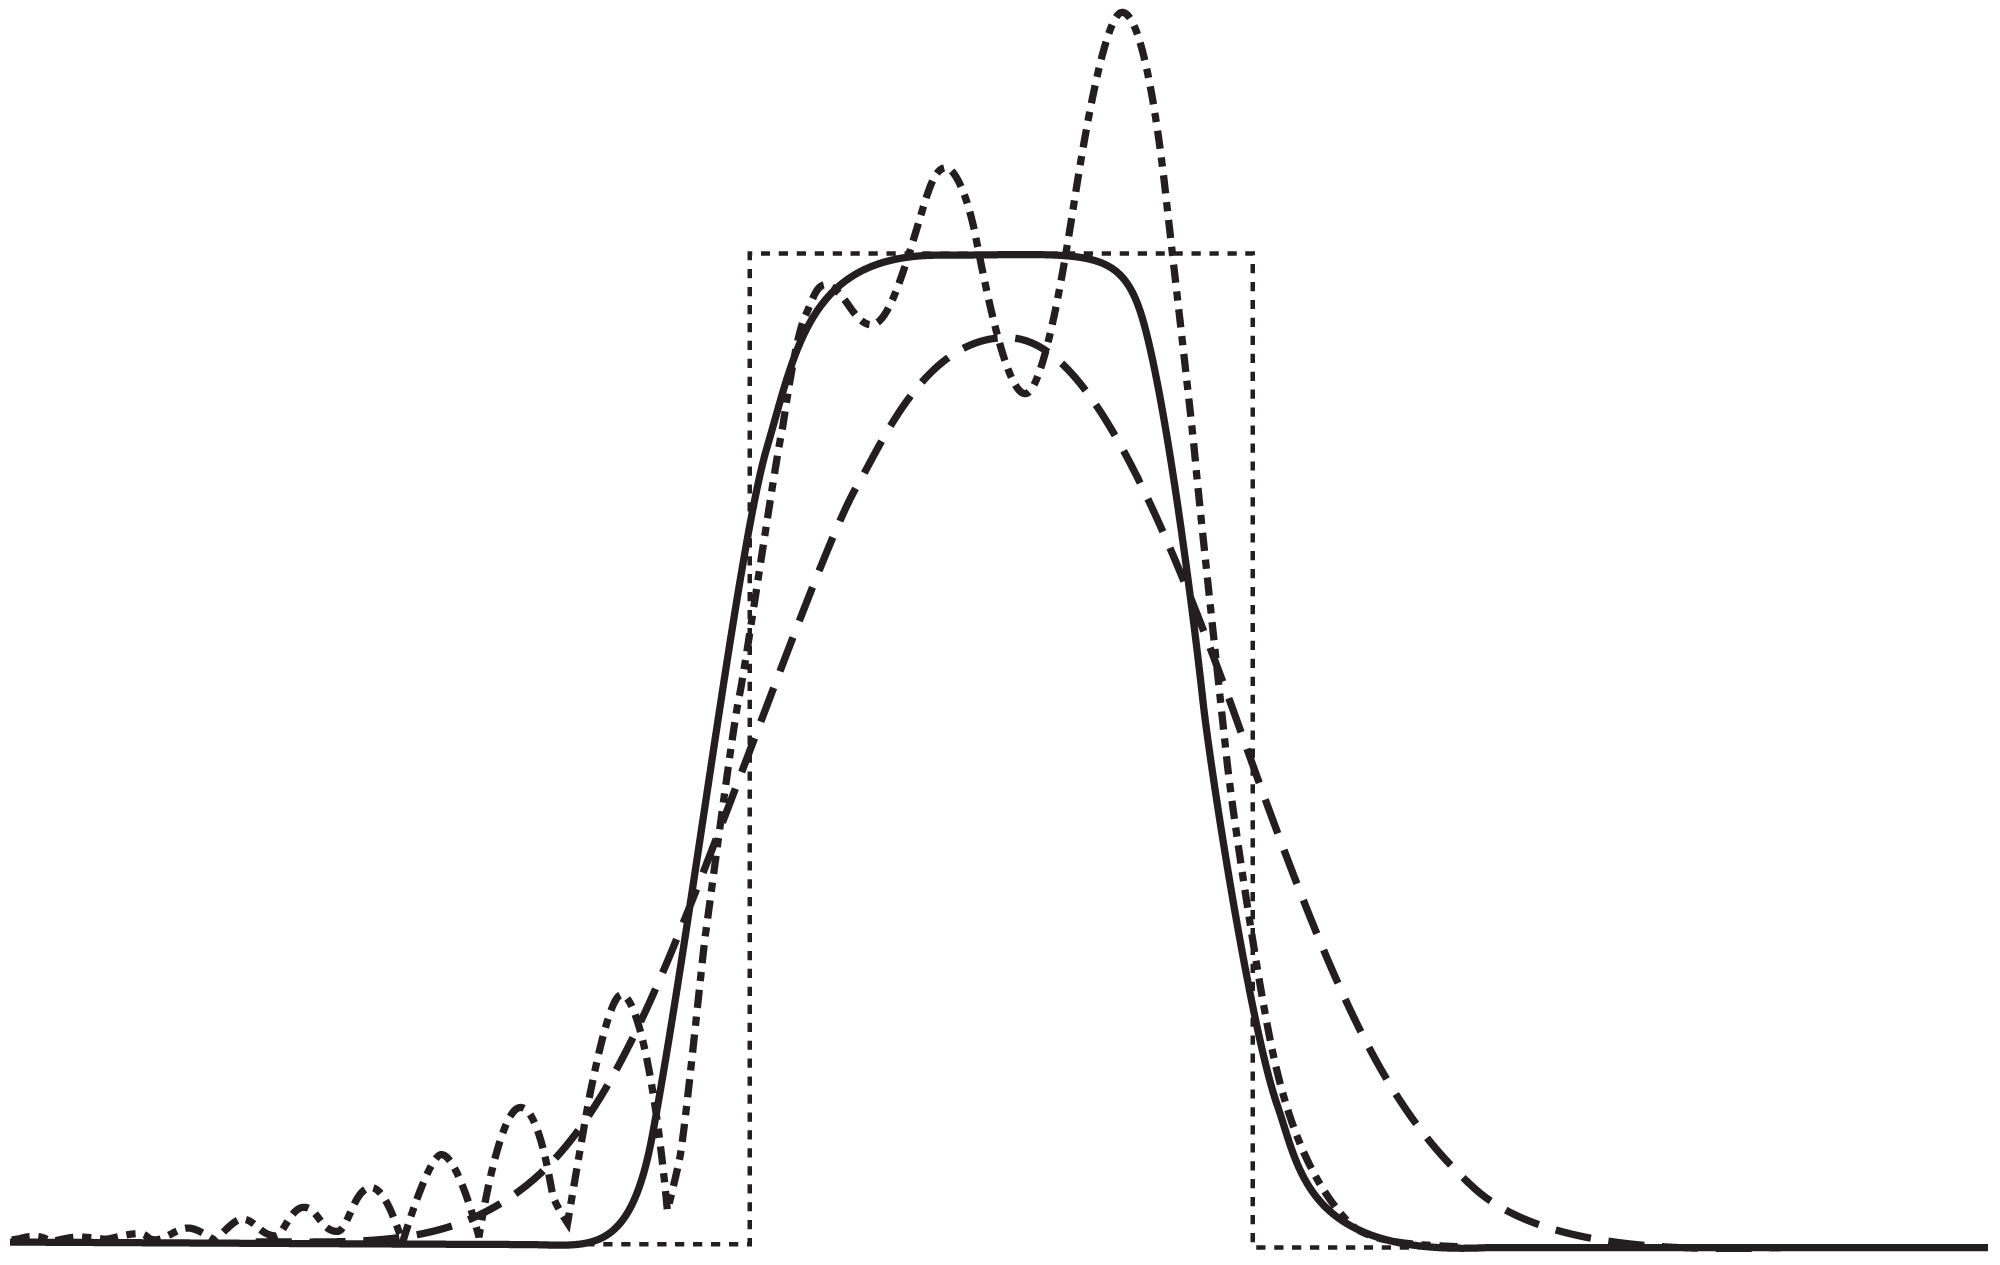
\includegraphics[width=0.75\textwidth]{png/hybrid-scheme-testing.png}}
\caption{Распространение прямоугольного импульса. Штриховая линия -- решение по схеме Куранта-Изаксона-Рис. Штрих-пунктирная -- решение по схеме Лакса-Вендрофа. Сплошная линия -- решение с использованием гибридной схемы. Точками показано точное решение.}
\label{pic:hybrid-scheme-testing}
\end{figure}
